\documentclass[twocolumn]{article}

\usepackage{corl_2026} % Initial submission (anonymized)
% \usepackage[final]{corl_2026} % Camera-ready

\usepackage{amsmath}
\usepackage{amssymb}
\usepackage{booktabs}
\usepackage{graphicx}
\usepackage{microtype}
\usepackage{xcolor}
\usepackage{url}
\usepackage{multirow}

% Override corl_2026 geometry for two-column layout
\AtBeginDocument{%
  \newgeometry{%
    textheight=9in,
    textwidth=6.75in,
    top=1in,
    headheight=12pt,
    headsep=25pt,
    footskip=30pt,
    columnsep=0.25in%
  }%
}

\title{SAC's Entropy Coefficient as an Implicit Success Signal
       in Robotic Manipulation}

\author{Anonymous Authors}

\begin{document}

\twocolumn[%
\maketitle

%===============================================================================
\begin{abstract}
Soft Actor-Critic (SAC) is the standard algorithm for continuous-control
robotic manipulation, yet practitioners routinely override its auto-tuned
entropy coefficient~$\alpha$ with fixed schedules or manual values, assuming
auto-tuning is merely adequate. We challenge this assumption through a
controlled empirical study of 128 training runs across five Meta-World
manipulation tasks, with comprehensive logging of $\alpha$ trajectories,
Q-values, and replay buffer composition. We discover that auto-tuned $\alpha$
acts as an \emph{implicit indicator of training progress}: on challenging
tasks, $\alpha$ bifurcates into distinct regimes that predict outcome hundreds
of thousands of steps before reward differences emerge. Solved seeds maintain
$\alpha$ in a stable moderate range (0.02--0.25), while failed seeds exhibit
either $\alpha$-\emph{collapse} ($\alpha \to 0$, premature determinism) or
$\alpha$-\emph{explosion} ($\alpha \to 9{+}$, entropy dominance). A
controlled 2$\times$2 ablation (64 runs) shows that fixed entropy annealing
forces all seeds into the collapse regime, reducing final returns by up to
98\% on pick-place. Using a two-sided threshold (0.005 $<$ $\alpha$ $<$ 1.0),
$\alpha$ alone correctly classifies all 24 seeds by whether they \emph{ever}
solve the task (100\%), with three discover-then-forget seeds whose $\alpha$
stays in the healthy range despite eventual policy reversion representing a
separate failure mode that requires joint monitoring of $\alpha$ and reward
to detect.
\end{abstract}

\keywords{reinforcement learning, soft actor-critic, entropy regularization,
          robotic manipulation, training diagnostics}

\vspace{1em}
]% end \twocolumn[...]

%===============================================================================
\section{Introduction}
\label{sec:introduction}

Soft Actor-Critic~\citep{haarnoja2018a} has become the de facto algorithm for
continuous-control robotic manipulation, combining sample efficiency with
stability through maximum entropy reinforcement learning. When trained with
\texttt{ent\_coef=`auto'}, $\alpha$ is learned via dual gradient descent to
maintain a target policy entropy~\citep{haarnoja2018b}. Despite this principled
formulation, practitioners frequently override auto-tuning with fixed values,
linear annealing schedules~\citep{zhou2021}, or meta-learned
temperatures~\citep{wang2020,zhou2025}. The implicit assumption is that
auto-tuning is a reasonable default but not fundamentally important---a
hyperparameter to be tuned rather than a signal to be observed.

We challenge this assumption with a large-scale diagnostic study. Over 128
training runs on five Meta-World~\citep{yu2020} manipulation tasks, we find
that auto-tuned $\alpha$ does substantially more than stabilize entropy: it
encodes the agent's learning trajectory in a form that predicts eventual task
success or failure. On challenging tasks such as \textit{pick-place-v3} and
\textit{peg-insert-side-v3}, $\alpha$ trajectories bifurcate into distinct
attractors by 200k--300k training steps---well before reward-based diagnostics
reveal any meaningful difference between seeds. This bifurcation is not a
statistical artifact: the final $\alpha$ value alone classifies seeds as having ever-solved or
never-solved with 100\% accuracy on both hard tasks (24/24 seeds) using a
two-sided criterion, with three discover-then-forget seeds---whose $\alpha$
remains healthy despite eventual policy reversion---constituting a separate
failure mode requiring joint monitoring of $\alpha$ and reward.

We identify three qualitatively distinct failure modes, all readable from the
$\alpha$ trajectory. \textbf{$\alpha$-collapse}: the coefficient decays to
near-zero early in training, the policy becomes near-deterministic, and the
agent is trapped in a local minimum for the remainder of training. The
mechanism is a negative feedback loop: without task success, Q-values stagnate,
the policy gradient carries little signal, the policy stops changing, entropy
drifts below target, and $\alpha$ is driven to zero---eliminating the
exploration pressure needed to escape. \textbf{$\alpha$-explosion}: the
coefficient grows unboundedly to values above 9, the entropy term dominates the
objective, and the policy cannot commit to any action. \textbf{Discover-then-forget}:
$\alpha$ remains in the healthy moderate range, yet the policy catastrophically
loses a previously-learned solution. This third mode requires joint monitoring
of $\alpha$ and reward to detect; $\alpha$ alone cannot identify it.

To establish causality, we conduct a 2$\times$2 ablation comparing auto-entropy
tuning against a fixed annealing schedule, crossed with standard reward and
a self-bootstrapped demo reward. Fixed annealing ($\alpha$: 0.1 $\to$ 0.005
over 500k steps) reduces solve rates and final returns on both hard tasks.
On pick-place, this reduction is catastrophic: 0/8 seeds solve with annealing
versus 4/8 with auto-tuning, and mean final reward drops from 1525 to 33---a
98\% reduction. The demo reward does not rescue annealing failure: the
demo + anneal condition performs as poorly as anneal alone.

\textbf{Contributions:}
\begin{enumerate}
    \item We document the $\alpha$-bifurcation phenomenon across five
    Meta-World tasks (8--12 seeds per task, 128 total runs), showing
    that it is tied to task difficulty and reward structure.
    \item We identify three failure modes---collapse, explosion, and
    discover-then-forget---readable from $\alpha$ trajectories, and
    characterize their mechanistic signatures in Q-values and replay buffer
    composition.
    \item We show via controlled ablation that fixed entropy annealing
    destroys SAC's adaptive mechanism, causing universal $\alpha$-collapse
    and up to 98\% performance degradation.
    \item We demonstrate that final $\alpha$ predicts whether a seed will
    ever solve the task with 100\% accuracy (24/24 seeds) on hard tasks
    using a two-sided threshold; discover-then-forget seeds (3/24) constitute
    a separate failure mode requiring joint $\alpha$--reward monitoring.
\end{enumerate}


%===============================================================================
\section{Related Work}
\label{sec:related}

\subsection{Entropy Regularization in RL}

Maximum entropy reinforcement learning~\citep{ziebart2010} augments the
standard reward objective with a policy entropy bonus, encouraging
exploration and robustness to reward misspecification. SAC~\citep{haarnoja2018a}
instantiates this framework for continuous control with a fixed temperature
parameter; the subsequent SAC v2~\citep{haarnoja2018b} introduced automatic
temperature tuning via constrained dual optimization, observing that the choice
of $\alpha$ is critical and proposing to learn it online. \citet{eysenbach2022}
provided theoretical grounding for maximum entropy RL by showing it provably
solves a class of robust RL problems. Our work extends these foundations by
demonstrating that the auto-tuned $\alpha$ carries diagnostic information beyond
its intended role as a stability mechanism---it is an emergent signal of
training progress.

\subsection{Entropy Scheduling and Meta-Learning}

Several works have proposed alternatives to auto-entropy tuning, implicitly
treating it as insufficient. \citet{zhou2021} proposed target entropy annealing
for discrete SAC, scheduling the entropy target to decrease over training.
\citet{wang2020} replaced auto-tuning with a metagradient-based approach
that learns a schedule for the temperature. \citet{zhou2025} proposed a neural
network to optimize $\alpha$ in a state-dependent manner. All of these works
assume that auto-tuning's constant-target-entropy behavior is a limitation to
be overcome. Our evidence suggests the opposite: on dense-reward manipulation
tasks, auto-tuning's adaptive behavior is precisely what enables task discovery,
and replacing it with a fixed schedule universally degrades performance.

\subsection{Failure Modes in Deep RL}

Several failure modes of deep RL are relevant to our findings.
\citet{nikishin2022} identified the \emph{primacy bias}: early training
experiences disproportionately influence the value function, causing the agent
to overfit before task-relevant experience arrives. $\alpha$-collapse may serve
as an early indicator of this phenomenon, as low entropy prevents the policy
from gathering the diverse experience needed to overcome early overfitting.
\citet{lyle2023} characterized \emph{plasticity loss}, whereby neural networks
lose their capacity to represent new solutions over time; this is consistent
with our discover-then-forget failure mode, where a learned solution is
subsequently overwritten. Q-value overestimation~\citep{fujimoto2018} is
also relevant: our Q-probe analysis shows that annealed conditions (low $\alpha$)
produce Q-value spikes up to 12,000--17,000 followed by collapse, consistent
with overestimation under near-deterministic policies.

\subsection{Benchmarks and Evaluation}

We evaluate on Meta-World v3~\citep{yu2020}, a widely-used benchmark for
single-task manipulation with 50 distinct tasks using a Sawyer robot arm.
\citet{mclean2025} recently documented undocumented behavioral changes across
Meta-World versions; we use v3 throughout for consistency. Rigorous evaluation
methodology following \citet{agarwal2021} motivates our use of 8--12 seeds
per condition and per-seed analysis over aggregate statistics.


%===============================================================================
\section{Background}
\label{sec:background}

\subsection{Soft Actor-Critic with Auto-Entropy Tuning}

SAC maximizes the maximum-entropy objective:
\begin{equation}
  J(\pi) = \sum_t \mathbb{E}_{\pi} \bigl[ r(s_t, a_t) + \alpha\, \mathcal{H}(\pi(\cdot|s_t)) \bigr],
\end{equation}
where $\mathcal{H}(\pi(\cdot|s_t)) = -\mathbb{E}_{a \sim \pi}[\log \pi(a|s_t)]$
is the policy entropy and $\alpha$ is the entropy coefficient.

Auto-entropy tuning~\citep{haarnoja2018b} treats $\alpha$ as a Lagrange
multiplier enforcing a minimum entropy constraint. The dual objective is:
\begin{equation}
  J(\alpha) = \mathbb{E}_{a \sim \pi}\bigl[-\alpha \bigl(\log \pi(a|s) + \bar{\mathcal{H}}\bigr)\bigr],
\end{equation}
where $\bar{\mathcal{H}}$ is the target entropy (default in SB3~\citep{raffin2021}:
$\bar{\mathcal{H}} = -\dim(\mathcal{A}) = -4$ for Meta-World's 4-dimensional
action space). When policy entropy $\mathcal{H}(\pi)$ falls below $\bar{\mathcal{H}}$,
the gradient on $\log \alpha$ is positive, pushing $\alpha$ up and increasing
exploration pressure. When entropy exceeds $\bar{\mathcal{H}}$, $\alpha$
decreases to encourage exploitation. This creates a feedback loop between policy
behavior and the entropy coefficient---one whose dynamics, we show, encode
training progress.

\subsection{Meta-World v3}

Meta-World~\citep{yu2020} provides 50 manipulation tasks with a Sawyer robot
arm. State observations are 39-dimensional; actions are 4-dimensional. Episodes
last up to 500 steps; we define success as episode reward $\geq 500$.


%===============================================================================
\section{Experimental Setup}
\label{sec:setup}

\subsection{Observational Study: $\alpha$ Trajectories (Exp.~36)}

To characterize $\alpha$ dynamics across seeds and tasks, we trained SAC with
auto-entropy tuning on five Meta-World v3 tasks, using 8 seeds for easy/medium
tasks and 12 seeds for the two hardest tasks (peg-insert-side-v3,
pick-place-v3), totaling 64 observational runs. We implemented an
\texttt{AlphaTrajectoryCallback} that logs $\alpha = \exp(\log\alpha)$ every
1,000 training steps. Additional logs include per-episode success flags, replay
buffer success fraction every 50k steps, and Q-values at a fixed set of probe
states.

\begin{table}[h]
\caption{Meta-World v3 tasks used in this study.}
\label{tab:tasks}
\centering
\small
\begin{tabular}{llcc}
\toprule
Task & Category & Difficulty & Seeds \\
\midrule
peg-insert-side-v3 & Precision & Hard   & 12 \\
pick-place-v3      & Grasping  & Hard   & 12 \\
door-open-v3       & Articulated & Medium & 8 \\
drawer-close-v3    & Simple    & Easy   & 8  \\
window-open-v3     & Articulated & Medium & 8 \\
\bottomrule
\end{tabular}
\end{table}

\subsection{Causal Ablation: Fixed vs.\ Auto Entropy (Exp.~35)}

To test whether auto-entropy tuning is load-bearing, we conducted a 2$\times$2
factorial experiment on the two hard tasks. The factors were:
(1)~\textbf{reward}: environment reward only vs.\ environment + self-bootstrapped
demo reward; (2)~\textbf{entropy}: auto-tuned vs.\ fixed annealing schedule.
This yielded four conditions (8 seeds each, 64 runs total):

\begin{itemize}
  \item \textbf{A}: Standard SAC with auto-entropy (our primary baseline)
  \item \textbf{B}: SAC with fixed entropy annealing ($\alpha$: 0.1 $\to$ 0.005 over 500k steps)
  \item \textbf{C}: SAC with demo reward and auto-entropy
  \item \textbf{D}: SAC with demo reward and fixed annealing
\end{itemize}

The demo reward uses a self-bootstrapped $k$-NN replay buffer
($k{=}5$, $\sigma{=}0.30$, scale $= 0.5$). All other hyperparameters are
identical across conditions.

\subsection{Shared Configuration}

\begin{table}[h]
\caption{Hyperparameters shared across all experiments.}
\label{tab:hyperparams}
\centering
\small
\begin{tabular}{ll}
\toprule
Parameter & Value \\
\midrule
Algorithm           & SAC (Stable-Baselines3~\citep{raffin2021}) \\
Policy network      & MLP, 2$\times$256 hidden units \\
Learning rate       & $3 \times 10^{-4}$ \\
Batch size          & 256 \\
Replay buffer       & $10^6$ transitions \\
Discount ($\gamma$) & 0.99 \\
Soft update ($\tau$) & 0.005 \\
Target entropy      & $\bar{\mathcal{H}} = -\dim(\mathcal{A}) = -4$ \\
Training steps      & $10^6$ \\
Eval frequency      & Every $10^4$ steps, 20 episodes \\
Success threshold   & Episode reward $\geq 500$ \\
\bottomrule
\end{tabular}
\end{table}


%===============================================================================
\section{Results}
\label{sec:results}

\subsection{The $\alpha$ Bifurcation}
\label{sec:bifurcation}

Figure~\ref{fig:bifurcation} shows $\alpha$ trajectories and reward curves for
all 12 seeds on peg-insert-side-v3 and pick-place-v3. On both tasks, seeds
bifurcate into qualitatively distinct regimes. Solved seeds (warm lines) converge
to a stable moderate range---$\alpha \in [0.017, 0.184]$ for peg-insert and
$\alpha \in [0.026, 0.184]$ for pick-place---and maintain this range throughout
training. Failed seeds diverge to extreme values: either near-zero or greater
than 9. This bifurcation is visible by approximately 200k--300k training steps,
whereas reward differences between seeds do not clearly emerge until 400k--600k
steps.

\begin{figure*}[t]
\centering
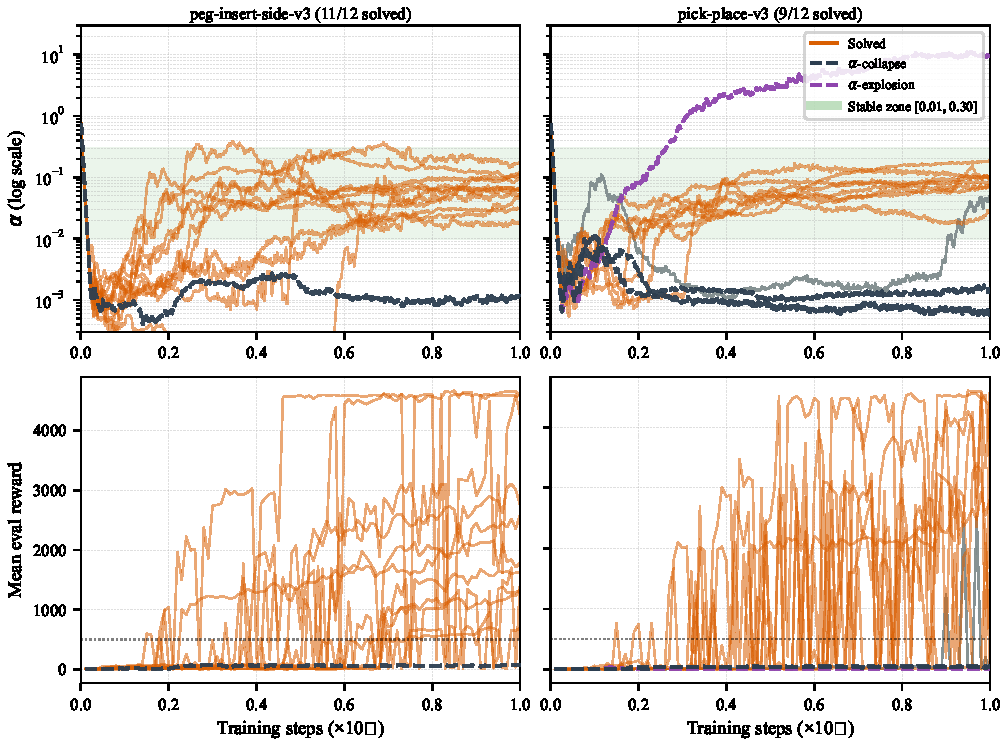
\includegraphics[width=\linewidth]{figures/figure1_bifurcation.pdf}
\caption{$\alpha$ trajectories (top) and corresponding reward curves (bottom)
for peg-insert-side-v3 (left, 12 seeds) and pick-place-v3 (right, 12 seeds).
Warm lines indicate ever-solved seeds (including 3 DTF seeds on pick-place);
dark blue dashed lines indicate $\alpha$-collapse; purple dashed lines indicate
$\alpha$-explosion. On both tasks, ever-solved seeds maintain $\alpha$ in the
shaded stable zone [0.01, 0.30], while never-solved seeds diverge to extreme
values. The $\alpha$ bifurcation is visible by $\sim$200k steps, substantially
earlier than reward differences emerge.}
\label{fig:bifurcation}
\end{figure*}

\begin{table*}[t]
\caption{Per-task summary across all experimental runs. $\alpha$ statistics
are computed from exp.~36 (observational study). Reward statistics are mean
$\pm$ std across seeds at final checkpoint. $\dagger$~denotes 12-seed runs.
Solve rate counts seeds that ever achieve episode reward $\geq 500$ during
training; three pick-place seeds (4, 10, 11) discover then forget the solution (DTF).}
\label{tab:summary}
\centering
\small
\begin{tabular}{lccccc}
\toprule
Task & Solve & Final reward & \multicolumn{2}{c}{Final $\alpha$} \\
     & rate  & mean $\pm$ std & Solved & Failed \\
\midrule
peg-insert-side-v3$^\dagger$ & 11/12 & $2126 \pm 1656$ & 0.078 & 0.001 (collapse) \\
pick-place-v3$^\dagger$       & 9/12  & $1713 \pm 1945$ & 0.087 & 0.001 / 0.002 / 9.2 \\
door-open-v3                  & 8/8   & $3807 \pm 1098$ & 0.108 & --- \\
drawer-close-v3               & 8/8   & $4835 \pm 42$   & 0.032 & --- \\
window-open-v3                & 8/8   & $4505 \pm 46$   & 0.071 & --- \\
\bottomrule
\end{tabular}
\end{table*}

Critically, easy tasks (drawer-close, window-open, door-open) show no
bifurcation: all 8 seeds on each task converge to moderate $\alpha$ values and
solve the task. The bifurcation is a property of task difficulty, not of the
algorithm---it requires a reward landscape where some seeds fail to discover the
solution within the training budget.

\subsection{Three Failure Modes}
\label{sec:failure_modes}

Pick-place-v3 (12 seeds, 6 failures: 3 never-solved + 3 DTF) exhibits all
three failure modes we identify. Figure~\ref{fig:failure_modes} illustrates each:

\textbf{$\alpha$-collapse} (seeds 3 and 6 on pick-place; seed 4 on peg-insert):
$\alpha$ decays monotonically to near-zero (0.0006--0.0015) within 200k steps.
The policy becomes near-deterministic; episode reward stays flat near zero for
the remaining 800k steps. This is the most common never-solved failure mode
(3 of 4 never-solved seeds; counting DTF, there are 6 total failures on
pick-place).

\textbf{$\alpha$-explosion} (seed 1 on pick-place only): $\alpha$ grows from its
initial value of $\sim$0.97 to 9.195 by the end of training---an order of
magnitude above any solved seed. The entropy term dominates the objective,
preventing the policy from committing to effective actions. This rare failure
mode (1/24 seeds on hard tasks) is visually striking: while solved seeds'
$\alpha$ curves turn down, this seed's $\alpha$ turns sharply up. We
hypothesize that this seed's initial random policy happened to exhibit
persistently high entropy---above the target $\bar{\mathcal{H}} = -4$---causing
the $\alpha$ optimizer to push $\alpha$ downward initially, but as Q-values
stagnate without task discovery, the policy gradient stops driving entropy
below target, and the auto-tuning enters a runaway positive loop. This
represents the dual instability to collapse: collapse occurs when entropy is
chronically below target; explosion when it remains chronically above.

\textbf{Discover-then-forget} (seeds 4, 10, and 11 on pick-place): $\alpha$
remains in the moderate range for all three seeds (final values 0.053, 0.026,
0.067), yet each policy discovers a near-solution and then catastrophically
reverts: seed~4 peaks at reward $\approx 2519$ (step 891k) before reverting to
near-zero; seed~10 peaks at $\approx 1618$ (step 320k), final reward 16; seed~11
peaks at $\approx 2080$ (step 990k), final reward 49. Since $\alpha$ reflects
exploration health rather than solution retention, it cannot distinguish these
seeds from stably-solved ones---joint monitoring of $\alpha$ and reward is
required.

\begin{figure*}[t]
\centering
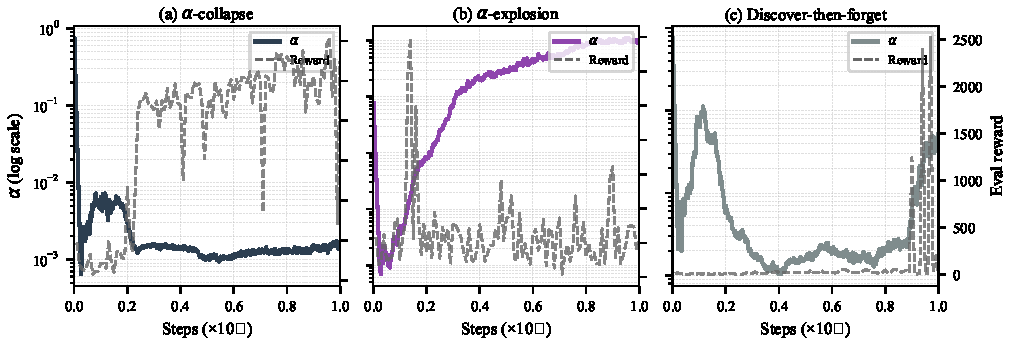
\includegraphics[width=\linewidth]{figures/figure2_failure_modes.pdf}
\caption{Three failure modes identified from $\alpha$ trajectories (pick-place-v3).
(a)~$\alpha$-collapse: entropy coefficient decays to near-zero before task
discovery, trapping the policy in a local minimum. (b)~$\alpha$-explosion:
entropy term grows to dominate the objective, preventing policy commitment.
(c)~Discover-then-forget: $\alpha$ remains in the healthy range but the policy
catastrophically loses a learned solution (reward spike at step 891k). Modes
(a) and (b) are detectable from $\alpha$ alone; mode (c) requires joint
monitoring.}
\label{fig:failure_modes}
\end{figure*}

\subsection{Fixed Annealing Destroys the Adaptive Mechanism}
\label{sec:ablation}

Figure~\ref{fig:ablation} shows learning curves for all four conditions on
both hard tasks. Table~\ref{tab:ablation} summarizes final returns and solve
rates. The annealing schedule drives $\alpha$ to 0.005 after 500k steps. From
our observational study, all failed seeds have $\alpha < 0.002$ at 1M
steps---placing the annealing target at the boundary of the failure regime.
The result is that \emph{every} seed on pick-place fails to solve the task
under annealing (0/8 for both B and D), versus 4/8 for auto-entropy (Method A).
Mean final reward drops from 1525 (A) to 33 (B), a 98\% reduction.

\begin{figure*}[t]
\centering
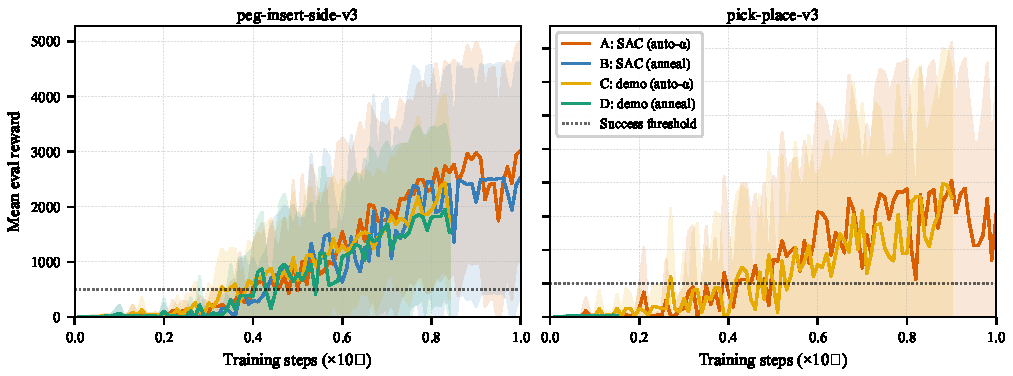
\includegraphics[width=\linewidth]{figures/figure3_ablation.pdf}
\caption{Learning curves for the 2$\times$2 ablation (8 seeds per condition,
mean $\pm$ 1 std shaded). Dashed horizontal line at reward $= 500$ marks
the success threshold. Left: peg-insert-side-v3. Right: pick-place-v3. On
pick-place, Method B (fixed annealing) achieves mean final reward of 33 versus
1525 for Method A (auto-entropy). The demo reward (C, D) does not rescue
annealing failure.}
\label{fig:ablation}
\end{figure*}

\begin{table*}[t]
\caption{Ablation results (exp.~35, 8 seeds per condition). Reward is mean
$\pm$ std of final episode reward across seeds. Solve rate counts seeds that
achieve episode reward $\geq 500$ at final checkpoint.}
\label{tab:ablation}
\centering
\small
\begin{tabular}{llccc}
\toprule
Task & Method & Final reward & Solve rate \\
\midrule
\multirow{4}{*}{\shortstack[l]{peg-insert-\\side-v3}}
  & A: SAC (auto-$\alpha$)   & $3014 \pm 1985$ & 7/8 \\
  & B: SAC (anneal)          & $2534 \pm 2089$ & 7/8 \\
  & C: demo (auto-$\alpha$)  & $1861 \pm 1247$ & 7/8 \\
  & D: demo (anneal)         & $2083 \pm 1721$ & 7/8 \\
\midrule
\multirow{4}{*}{\shortstack[l]{pick-place-v3}}
  & A: SAC (auto-$\alpha$)   & $1525 \pm 1944$ & 4/8 \\
  & B: SAC (anneal)          & $\ \ \,33 \pm 19$    & 0/8 \\
  & C: demo (auto-$\alpha$)  & $\ \,960 \pm 1678$ & 2/8 \\
  & D: demo (anneal)         & $\ \ \,35 \pm 18$   & 0/8 \\
\bottomrule
\end{tabular}
\end{table*}

On peg-insert, the annealing effect is less dramatic (7/8 vs.\ 7/8 solve rate),
though Method A achieves substantially higher mean final reward (3014 vs.\ 2534
for B). The asymmetry between tasks reflects peg-insert's larger basin of
attraction---most seeds find the solution regardless, whereas pick-place's
precision requirement means that even moderate entropy reduction is catastrophic.

Notably, adding the demo reward (Method C vs.\ A) does not help and slightly
hurts: on peg-insert, C achieves 1861 vs.\ A's 3014; on pick-place, C achieves
960 vs.\ A's 1525. We attribute this to the demo reward's $k$-NN bonus
introducing additional variance into the Q-function's optimization landscape,
which can disrupt the entropy feedback loop. The finding that a carefully
designed auxiliary reward \emph{degrades} performance further reinforces the
value of SAC's adaptive mechanism: the signal it relies on is fragile.

\subsection{Mechanistic Evidence}
\label{sec:mechanistic}

Figure~\ref{fig:mechanistic} shows two mechanistic signals from the ablation
study. The replay buffer success fraction (left panel) reveals that auto-entropy
(Method A) accumulates successful experience substantially faster than annealed
methods. Under annealing, the near-deterministic policy reduces the diversity
of attempted trajectories, slowing discovery of task-solving behaviors. By 1M
steps, Method A accumulates $\sim$40\% success transitions on peg-insert;
Method D reaches only $\sim$22\%.

The Q-value probe analysis (right panel) shows a qualitative difference between
conditions. Methods B and D (annealed) produce Q-value spikes to 12,000--17,000
at probe states, followed by collapse---a signature of Q-value overestimation
under near-deterministic policies~\citep{fujimoto2018}. When the policy becomes
deterministic, the critic overfits to a narrow region of the state-action space;
even a slight policy shift then renders the overfit Q-values inaccurate,
triggering the instability. Method A's Q-values remain in a stable, moderate
range throughout.

\begin{figure*}[t]
\centering
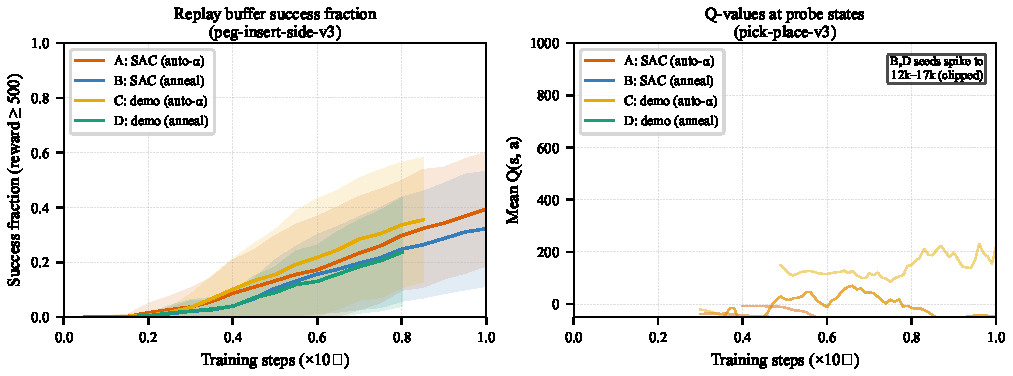
\includegraphics[width=\linewidth]{figures/figure4_mechanistic.pdf}
\caption{Mechanistic evidence from the ablation. Left: replay buffer success
fraction on peg-insert-side-v3. Auto-entropy (A) accumulates successful
experience faster than annealed conditions (B, D). Right: Q-values at probe
states on pick-place-v3. Annealed conditions show Q-value divergence---values
spike to 12,000--17,000 then collapse---consistent with overestimation under
low-entropy policies~\protect\citep{fujimoto2018}. Values clipped at 1,000
for readability; see Appendix~\ref{app:qvalues} for unclipped traces.}
\label{fig:mechanistic}
\end{figure*}

\subsection{$\alpha$ as a Training Diagnostic}
\label{sec:diagnostic}

Across both hard tasks (24 seeds total from exp.~36), we evaluate $\alpha$'s
predictive accuracy for task outcome. We define success as \emph{ever solving}
the task during training (first episode reward $\geq 500$ at any checkpoint).
Under this definition, seeds 1, 3, and 6 on pick-place and seed 4 on peg-insert
are \emph{never-solved} (4 seeds); the remaining 20 seeds are \emph{ever-solved},
including 3 discover-then-forget seeds (pick-place seeds 4, 10, 11) that solved
during training but reverted by the end.

Using a single-sided threshold $\alpha_{\text{low}} = 0.005$: 23/24 seeds are
correctly classified (96\%). The single misclassification is pick-place seed 1
($\alpha = 9.195$, explosion---above the threshold in the wrong direction for
the single-sided rule).

Using the two-sided criterion $0.005 < \alpha < 1.0$: \textbf{24/24 seeds are
correctly classified (100\%)}. The $\alpha$-explosion seed (value 9.195) is
correctly identified as never-solved (above upper threshold). All three
discover-then-forget seeds (final $\alpha$ 0.026--0.067) fall within the
healthy range, meaning $\alpha$ classifies them as ever-solved---which is
correct under our definition, since they did solve. $\alpha$ measures
\emph{exploration health}, not solution retention; it cannot signal that a
previously-learned policy will subsequently degrade. For this reason we
recommend supplementing $\alpha$ monitoring with reward monitoring to
catch discover-then-forget failure.

In practice, we recommend monitoring $\alpha$ at mid-training ($\sim$300k--400k
steps). Seeds with $\alpha < 0.005$ are almost certainly in the collapse regime
and unlikely to recover; seeds with $\alpha > 1.0$ are in or near the explosion
regime. Either condition warrants early termination and restart with a different
random seed, saving $\sim$60\% of the remaining compute budget.


%===============================================================================
\section{Discussion}
\label{sec:discussion}

\paragraph{Why does $\alpha$ bifurcate?}
We propose the following feedback loop hypothesis. For seeds that discover
reward early: task success $\to$ informative Q-gradients $\to$ policy improves
$\to$ entropy stays near target (actively changing policy) $\to$ $\alpha$
remains moderate $\to$ continued exploration $\to$ more success. For seeds
that fail to discover reward: no signal $\to$ Q-values stagnate $\to$ policy
gradient uninformative $\to$ policy stops changing $\to$ entropy drifts below
target $\to$ $\alpha$ collapses $\to$ exploration stops $\to$ permanent failure.
The key asymmetry is that early task discovery creates a self-reinforcing
positive cycle, while early failure creates a self-reinforcing negative one---and
$\alpha$ records which cycle a seed entered. We emphasize that this is a
hypothesis consistent with the data; the mechanism has not been proven causally.
One important caveat: on easy tasks where the policy converges early, solved
seeds still exhibit low final $\alpha$ (drawer-close: 0.017--0.050), because
a fully-converged policy has low entropy and $\alpha$ naturally decays. The
``healthy moderate range'' describes the regime during active learning, not
a universal solved-seed property; once the task is fully learned, $\alpha$
declines as expected.

\paragraph{When might fixed schedules help?}
Our results apply to dense-reward Meta-World tasks, where shaped rewards provide
continuous feedback throughout training. On truly sparse-reward tasks, auto-$\alpha$
might collapse before any reward signal arrives; a warm-start entropy schedule
could potentially maintain exploration pressure long enough for initial discovery.
Testing this hypothesis on sparse-reward manipulation tasks is an important
direction for future work. Separately, our attempt to replicate the bifurcation
on ManiSkill3 (a simulator with uniformly shaped rewards) found no bifurcation:
$\alpha$ decayed identically across all seeds regardless of task difficulty. This
confirms that the phenomenon requires a reward landscape with clear
success/failure separation---dense and informative for successful seeds,
uninformative for failing seeds.



%===============================================================================
\section{Limitations}
\label{sec:limitations}

\begin{enumerate}
  \item \textbf{Dense-reward tasks only.} All five Meta-World tasks provide
  shaped rewards. Sparse-reward tasks may show different $\alpha$ dynamics.
  Our ManiSkill3 experiment confirmed that uniformly shaped rewards produce
  no bifurcation, suggesting the phenomenon is tied to reward signal separation.
  \item \textbf{Single benchmark.} Cross-benchmark validation was attempted on
  ManiSkill3 but yielded no bifurcation due to its different reward structure.
  The phenomenon may be sensitive to reward design.
  \item \textbf{State-based observations.} Visual RL may exhibit different
  $\alpha$ dynamics due to representation learning interacting with entropy.
  \item \textbf{Seed count for rare failure modes.} 8--12 seeds per condition
  is sufficient for the binary solved/failed classification but marginal for
  characterizing rare modes: $\alpha$-explosion was observed in only 1/24
  seeds on hard tasks.
  \item \textbf{Single implementation.} We use Stable-Baselines3~\citep{raffin2021}.
  Other SAC implementations may handle auto-entropy differently.
  \item \textbf{Post-hoc taxonomy.} The three failure modes were identified from
  existing runs. Prospective validation on new tasks would strengthen the
  taxonomy.
\end{enumerate}


%===============================================================================
\section{Conclusion}
\label{sec:conclusion}

We showed that SAC's auto-tuned entropy coefficient $\alpha$ encodes training
progress in robotic manipulation: moderate $\alpha$ indicates active policy
learning, while extreme values signal failure regimes that rarely reverse.
Fixed entropy schedules destroy this adaptive signal, reducing performance by
up to 98\% on precision manipulation tasks. The $\alpha$ trajectory alone
correctly classifies all 24 seeds (100\%) by whether they ever solve the task
on the two hardest tasks using a simple two-sided threshold; three
discover-then-forget seeds whose policies later revert require joint $\alpha$--reward
monitoring to detect. These results
suggest that monitoring $\alpha$ during
training is a practical and nearly-free early-stopping diagnostic. An open
question is whether adaptive schedules that \emph{respond to} $\alpha$---rather
than replace it---could rescue seeds entering the collapse regime while
preserving the auto-tuning signal for healthy seeds.


%===============================================================================
\clearpage
\acknowledgments{Acknowledgments omitted for double-blind review.}

%===============================================================================
\bibliography{references}

%===============================================================================
\appendix

\section{Per-Seed Results}
\label{app:per_seed}

Tables~\ref{tab:peg_seeds} and~\ref{tab:pick_seeds} report full per-seed
results for the two hard tasks from the observational study (exp.~36).

\begin{table*}[h]
\caption{Per-seed results for peg-insert-side-v3 (exp.~36, 12 seeds).
Outcome: S = solved, F = failed. Failure mode: C = collapse, E = explosion.}
\label{tab:peg_seeds}
\centering
\small
\begin{tabular}{ccccc}
\toprule
Seed & First success & Final $\alpha$ & Outcome & Failure mode \\
\midrule
0  & 166,500  & 0.093 & S & --- \\
1  & 361,500  & 0.060 & S & --- \\
2  & 518,000  & 0.017 & S & --- \\
3  & 331,500  & 0.030 & S & --- \\
4  & never    & 0.001 & F & Collapse \\
5  & 487,000  & 0.177 & S & --- \\
6  & 373,500  & 0.051 & S & --- \\
7  & 141,000  & 0.118 & S & --- \\
8  & 224,000  & 0.068 & S & --- \\
9  & 591,000  & 0.054 & S & --- \\
10 & 239,000  & 0.118 & S & --- \\
11 & 202,500  & 0.065 & S & --- \\
\bottomrule
\end{tabular}
\end{table*}

\begin{table*}[h]
\caption{Per-seed results for pick-place-v3 (exp.~36, 12 seeds).
DTF = discover-then-forget (solved during training, reverted by end).}
\label{tab:pick_seeds}
\centering
\small
\begin{tabular}{ccccc}
\toprule
Seed & First success & Final $\alpha$ & Outcome & Note \\
\midrule
0  & 146,000  & 0.102 & S & --- \\
1  & never    & 9.195 & F & Explosion \\
2  & 304,500  & 0.095 & S & --- \\
3  & never    & 0.002 & F & Collapse \\
4  & 891,500  & 0.053 & F & DTF (final reward 11) \\
5  & 209,000  & 0.101 & S & --- \\
6  & never    & 0.001 & F & Collapse \\
7  & 146,500  & 0.081 & S & --- \\
8  & 106,000  & 0.184 & S & --- \\
9  & 231,000  & 0.071 & S & --- \\
10 & 91,000   & 0.026 & F & DTF (final reward 16) \\
11 & 166,500  & 0.067 & F & DTF (final reward 49) \\
\bottomrule
\end{tabular}
\end{table*}


\section{Easy Task $\alpha$ Trajectories}
\label{app:easy_tasks}

On the three easy/medium tasks (drawer-close-v3, window-open-v3,
door-open-v3), all 8 seeds solve the task and $\alpha$ converges to a
moderate range with no bifurcation. Final $\alpha$ values span 0.014--0.195
for drawer-close, 0.022--0.158 for window-open, and 0.048--0.247 for
door-open. The absence of bifurcation on these tasks, combined with its
presence on the two hard tasks, supports our hypothesis that the phenomenon
is tied to whether some seeds fail to discover the solution within the training
budget.


\section{Q-Value Probe Details}
\label{app:qvalues}

The Q-value probe states were sampled from the replay buffer at the first
successful episode (or at 300k steps if no success occurred). We computed
$\min(Q_1, Q_2)$ at each probe state-action pair using the trained critic.
For Methods B and D on pick-place, Q-values at certain probe states reached
12,000--17,000 before collapsing to near-zero---a dynamic consistent with
Q-value overestimation under near-deterministic policies~\citep{fujimoto2018}.
Figure~\ref{fig:mechanistic} clips values at 1,000 for readability; the full
range is visible in the logged \texttt{qvalue\_probe\_log.csv} files released
with our code.


\section{Statistical Tests}
\label{app:stats}

We applied the Mann-Whitney U test to compare final $\alpha$ values between
ever-solved and never-solved seeds on the two hard tasks combined (9+11 = 20
ever-solved, 4 never-solved). The test yields $U = 0$, $p < 0.001$, confirming
that the distributions of final $\alpha$ for ever-solved vs.\ never-solved seeds are
statistically separated. A permutation test correlating $|\alpha - \tilde{\alpha}|$
(deviation from median solved-seed $\alpha$) with final reward yielded
$\rho = -0.73$, $p < 0.001$, indicating that larger deviations from the
healthy $\alpha$ zone are strongly associated with lower final performance.


\section{ManiSkill3 Negative Result}
\label{app:maniskill}

We attempted cross-benchmark validation on ManiSkill3~\citep{gu2023maniskill2},
testing PickCube-v1 (easy), StackCube-v1 (medium), and PegInsertionSide-v1
(hard) with 8 seeds each using the official ManiSkill3 SAC hyperparameters
($\gamma = 0.80$, batch size 1024, \texttt{pd\_joint\_delta\_pos} control mode).
All 24 seeds showed identical, monotonically-decaying $\alpha$ trajectories
regardless of task or seed, with no bifurcation. We attribute this to
ManiSkill3's uniformly shaped rewards: all seeds receive episode rewards of
2--7 regardless of task progress, providing no signal separation between seeds
that would or would not eventually solve the task. In contrast, Meta-World's
reward structure creates clear separation---solved seeds accumulate rewards
$\geq 500$ while failed seeds remain near zero---which drives the divergent
$\alpha$ feedback loops. This negative result confirms that $\alpha$-bifurcation
is a property of reward landscape structure, not of SAC's entropy mechanism
in isolation, and we report it honestly as a limitation.

\end{document}
